\frame{
\frametitle {Desempenho}

\begin{table}[htb]\footnotesize
  \begin{center}
   \caption{Descri\c{c}\~{a}o do ambiente de simula\c{c}\~{a}o}.\label{tab:ambiente-simulacao}
    \begin{tabular}{l|l}
      \textbf{Processador} & Intel Core 2 Duo 2.53Mhz \\ \hline
      \textbf{Mem\'{o}ria RAM} & 4GB \\ \hline
      \textbf{Sistema Operacional} & Mac OS X 10.6.4 \\ \hline
      \textbf{Linguagem} & PHP 5.3 \\ \hline
      \textbf{SGDB} & MySQL 5.1 \\ \hline
      \textbf{Algoritmo de Hash} & SHA-1 \\ \hline
      \textbf{Tamanho de Chave HMAC} & 128 bits \\ \hline
      \textbf{Algoritmo de cifração} & AES 128 bits \\ \hline
      \textbf{Tamanho de chave sim\'{e}trica} & 128 bits \\
    \end{tabular}
  \end{center}
\end{table}

}

\frame{
\frametitle {Select, Insert, Updade e Delete}

\begin{figure}[ht]
\begin{center}
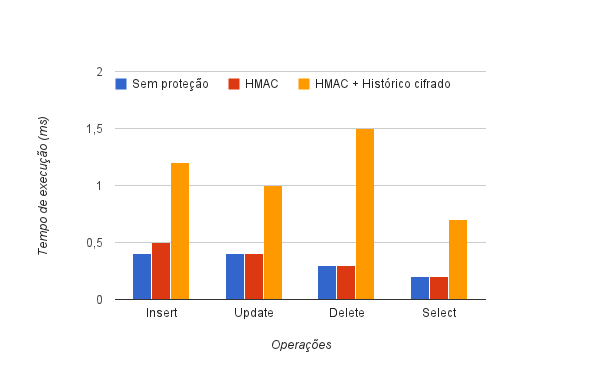
\includegraphics[width=\textwidth]{images/execucao1reg.png}
\caption{Tempo de execu\c{c}\~{a}o em segundos.} \label{figura:desempenho1reg}
\end{center}
\end{figure}

}

\frame{
\frametitle {Calculo em tabelas ja existentes}

\begin{figure}[ht]
\begin{center}
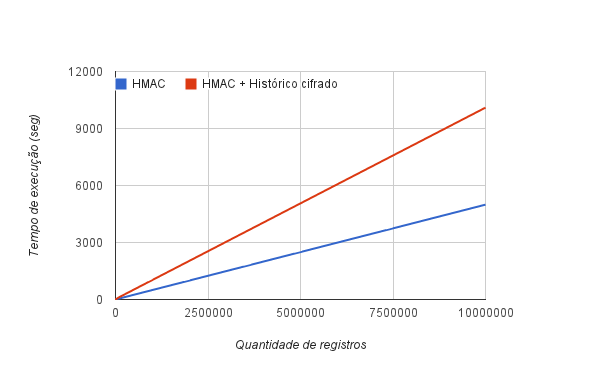
\includegraphics[width=\textwidth]{images/execucaoAdd.png}
\caption{Tempo de execu\c{c}\~{a}o em segundos.} \label{figura:desempenhoAdd}
\end{center}
\end{figure}

}

\frame{
\frametitle {Verificar integridade}

\begin{figure}[ht]
\begin{center}
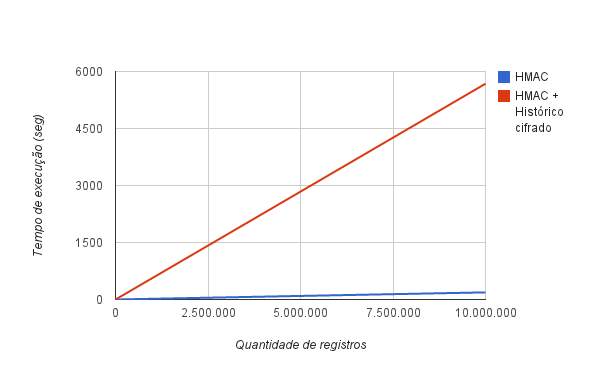
\includegraphics[width=\textwidth]{images/verificar.png}
\caption{Tempo de execu\c{c}\~{a}o em segundos.} \label{figura:verificar}
\end{center}
\end{figure}
}



